\section{商业模式战略}

商业模式战略领域:\textbf{商业模式环境}、\textbf{评估商业模式}、从商业模式的视角看\textbf{蓝海战略}的商业模式解读,以及如何在企业内部\textbf{管理多种商业模式}。

\subsection{商业模式环境}

日益复杂的经济环境(比如网络商业模式)、更大的不确定性(比如技术创新)和严峻的市场颠覆(比如经济动荡、颠覆性的新价值主张),这些都使得不断地审视环境比以前任何时候都重要。理解环境中的这些变化能帮助你把商业模式调整得更有效地化解外部力量。

\begin{figure}[H]
	\centering
	\vspace{-0.5em}
	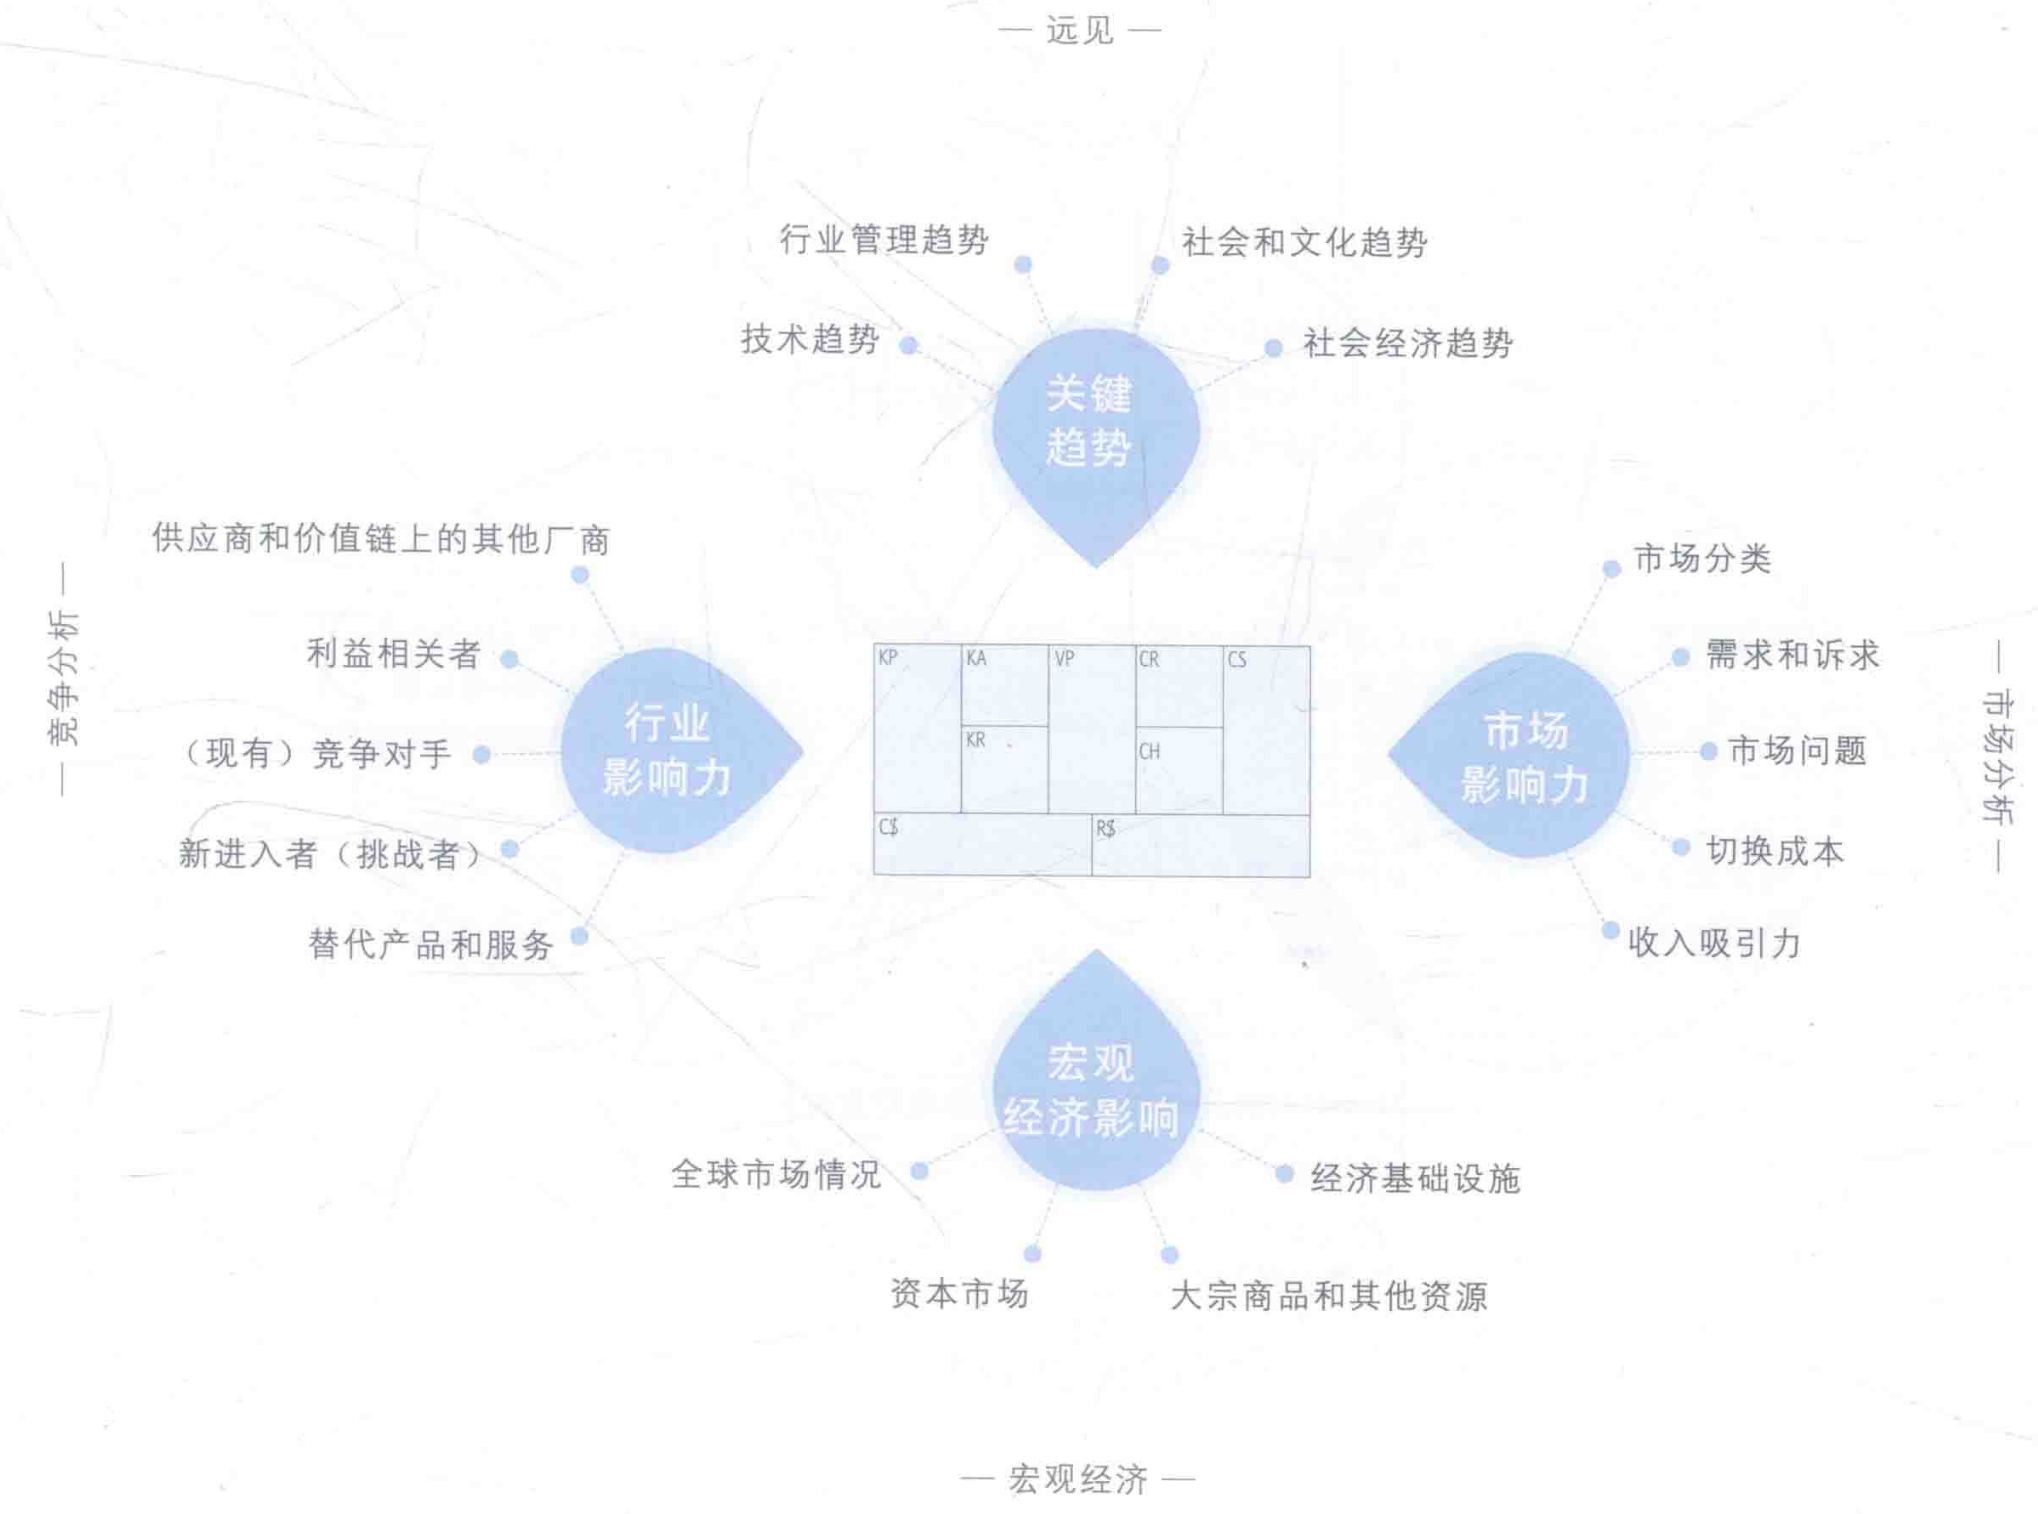
\includegraphics[width=0.8\textwidth]{img/商业模式环境评估.png}
    \vspace{-0.5em}
\end{figure}

\subsection{评估商业模式}

和年度体检一样,定期评估商业模式是一项重要的管理活动。这能让一个组织评估它的市场地位的健康程度,并且做出相应的调整。这种检查将成为商业模式不断进步的基础 ,或者也可能触发一次颠覆性的商业模式创新。
\begin{itemize}
    \item 某商业模式的总体评估,以及相应的未来战略
    \item 商业模式优势、劣势、机会和威胁(Strength, Weakness, Opportunity, Threat, SWOT)的检查清单(Checklist)
\end{itemize}

例:亚马逊总体商业模式评估
\begin{figure}[H]
	\centering
	\vspace{-0.5em}
	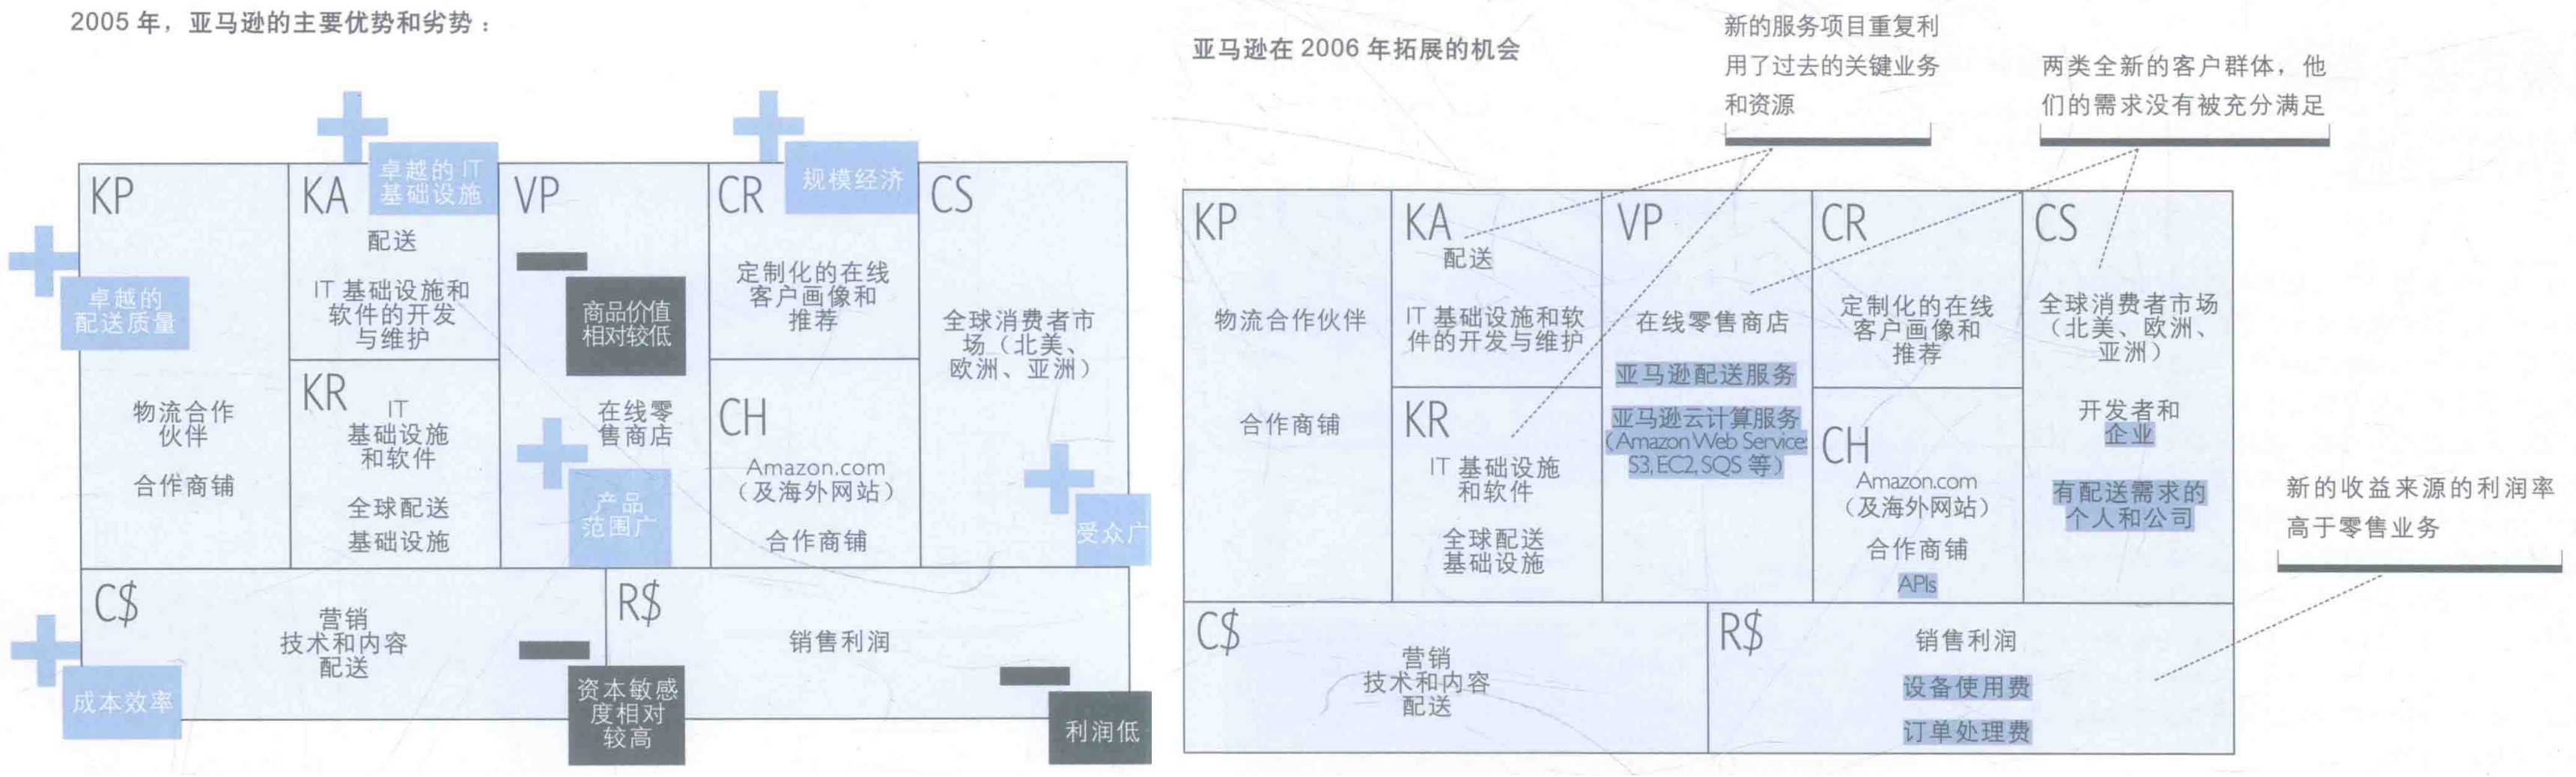
\includegraphics[width=\textwidth]{img/亚马逊总体商业模式评估.png}
    \vspace{-0.5em}
\end{figure}

对商业模式每个模块进行SWOT评估
\begin{itemize}
    \item SWOT分析是用来分析一个组织的优势和劣势,识别潜在的机会与威胁的工具。
    \item  SWOT问了四个简单的大问题。前两个——你的组织的优势和劣势是什么?内部评估你的组织。后两个——你的组织的机会有哪些,面临的潜在威胁又有哪些?在所处的环境下评估你的组织的位置。
\end{itemize}
\begin{figure}[H]
	\centering
	\vspace{-0.5em}
	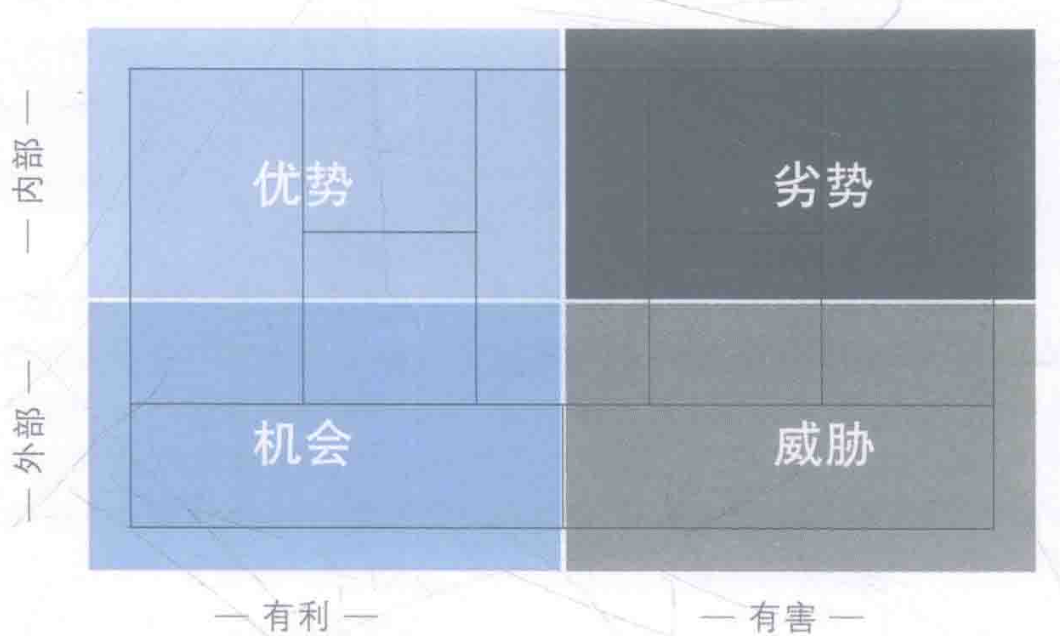
\includegraphics[width=0.5\textwidth]{img/SWOT评估.png}
    \vspace{-0.5em}
\end{figure}

优势劣势(SW)评估
\begin{multicols}{2}
\begin{itemize}
    \item 价值主张评估
    \begin{itemize}
        \item 我们的价值主张与客户需求一致
        \item 我们的价值主张具有很强的网络效应
        \item 在我们的产品和服务之间有很强的协同效应
        \item 我们的客户非常满意
    \end{itemize}
    \item 成本/收入评估
    \begin{itemize}
        \item 我们有较高的利润率
        \item 我们的收益是可预测的
        \item 我们有很多经常性收入,有很多回头客
        \item 我们的收入来源是多样化的
        \item 我们的收入来源是可持续的
        \item 我们在支出成本之前就有收入进账
        \item 客户真正想买的就是我们提供的
        \item 我们的定价机制可以抓住客户全部的购买意愿
        \item 我们的成本是可预测的
        \item 我们的成本结构与商业模式是完全匹配的
        \item 我们的运营低成本、高效率
        \item 我们受益于规模效应
    \end{itemize}
    \item 基础设施评估
    \begin{itemize}
        \item 竞争对手很难复制我们的核心资源
        \item 我们的资源需求是可预测的
        \item 我们在恰当的时间合理的调配核心资源
        \item 我们高效的执行了关键业务
        \item 我们的关键业务很难被复制
        \item 我们的执行质量很高
        \item 我们很好的平衡了自主业务和外包业务
        \item 我们专心致志,并且在必要的时候与合作伙伴合作
        \item 我们和重要合作伙伴的工作关系十分融洽
    \end{itemize}
    \item 客户界面评估
    \begin{itemize}
        \item 我们的客户的流失率很低
        \item 我们很好的细分了客户群体
        \item 我们不断的获得新的客户
        \item 我们的渠道通路很有效率
        \item 我们的渠道通路设置合理
        \item 我们的渠道通路与客户群是强接触的
        \item 我们的客户很容易就能看到我们的渠道通路
        \item 我们的渠道通路被高度整合
        \item 我们的渠道通路创造出了范围效应
        \item 我们的渠道通路很好的匹配了客户群体
        \item 我们有良好的客户关系
        \item 我们的客户关系品质与客户群体相匹配
        \item 客户切换的成本很高,客户与我们绑定了关系
        \item 我们的品牌很强
    \end{itemize}
\end{itemize}
\end{multicols}


评估机会(O)
\begin{itemize}
    \item 价值主张中的机会(整合、服务化与拓展)
    \begin{itemize}
        \item VP:产品与服务能否整合,产品能否服务化?价值主张的补充和外延?满足客户的额外需求或其它可做的工作?
    \end{itemize}
    \item 成本/收入中的机会(可重复、交叉销售、开源节流)
    \begin{itemize}
        \item  R\$:重复性收入代替一次性收入、寻找额外买单元素与交叉销售的机会、新的收益来源、能否提价
        \begin{itemize}
            \item 交叉销售:通过客户关系管理发现现有顾客的多种需求,并通过满足其需求而销售多种相关服务或产品的一种新兴营销方式
        \end{itemize}
        \item C\$:成本削减
    \end{itemize}
    \item 基础设施中的机会(强化核心、减轻负担、转让闲置)
    \begin{itemize}
        \item KR:核心资源的降本、外包、强化、转让
        \item KA:标准化、IT技术带来的整体效率提升
        \item KP:外包与核心业务聚焦、交叉销售与更好的客户连接、价值主张补充
    \end{itemize}
    \item 客户界面的机会(增长的市场、客户细分、渠道优化与去中间商,客户关系加强与取舍)
    \begin{itemize}
        \item CS:找到增长的市场并从中获利、服务新客户群体或更细致的已有客户分类
        \item CH:渠道的效率、效益、整合,补充性的渠道伙伴,去中间商、渠道客户匹配
        \item CR:加强与客户的关系并提升客户跟进的效果、定制化或可自动维护、提升切换成本、是否抛弃没有利润的客户以及原因  
    \end{itemize}
\end{itemize}

评估威胁(T)
\begin{itemize}
    \item 对价值主张的威胁(可替代性)
    \begin{itemize}
        \item 产品是否可替代?
        \item 是否会被更有竞争力的价格或更好的价值取代?
    \end{itemize}
    \item 对成本/收入的威胁(利润的威胁、是否单一、缩水、无法预测、无法支撑)
    \begin{itemize}
        \item 受威胁的利润?是否是技术原因导致?
        \item 是否过度依赖某一项或多项收益来源?
        \item 未来可能消失(或缩水)的收益来源?
        \item 是否有无法预测的成本?
        \item 哪些成本的增加会快过它们所支撑的收入?
    \end{itemize}
    \item 对基础设施的威胁(供应不足、干扰、合作关系波动)
    \begin{itemize}
        \item KR:某些资源的供应短缺?资源的质量是否有保证?
        \item KA:哪些关键业务会被打扰?我们的活动质量能否保证?
        \item KP:可能失去的合作伙伴?是否会跟竞争对手合作?是否过分依赖某些合作伙伴?
    \end{itemize}
    \item 客户界面上的威胁(市场竞争、渠道威胁、客户关系恶化)
    \begin{itemize}
        \item CS:市场是否很快饱和?市场份额被友商威胁?客户转投的可能性?竞争白热化的速度?
        \item CH:竞争对手是否威胁渠道?是否存在渠道与客户不相关的危险?
        \item CR:我们的客户关系有可能恶化吗?
    \end{itemize}
\end{itemize}


\subsection{蓝海战略}

蓝海战略是通过根本性的差异化来创造全新的行业,而不是通过模仿现有商业模式在当前行业中竞争。
\begin{itemize}
    \item 相对于在传统的绩效指标下超越对手,更加倡导创造新的、未充分竞争的市场空间,这称之为价值创新
    \begin{itemize}
        \item 这意味着通过创造新的利益和服务来为客户增加价值,同时通过削减低价值的功能或服务来降低成本。
        \item 为了实现价值创新,提出了“四项行动架构”。以 四个关键问题可以挑战一个行业的战略逻辑和现行的商业模式:
        \begin{itemize}
            \item 行业中哪些看起来理所当然的要素应该被删除?
            \item 哪些要素应该被大幅削减到行业标准之下?
            \item 哪些要素应该大幅提升到行业标准之上?
            \item 哪些行业中从未提供的要素是应该被创造出来的?
        \end{itemize}
    \end{itemize}
    \item 除了价值创新,还建议开拓未被开发的客户群体,以此来创造蓝海和发现新的市场。
\end{itemize}

\begin{figure}[H]
	\centering
	\vspace{-0.5em}
	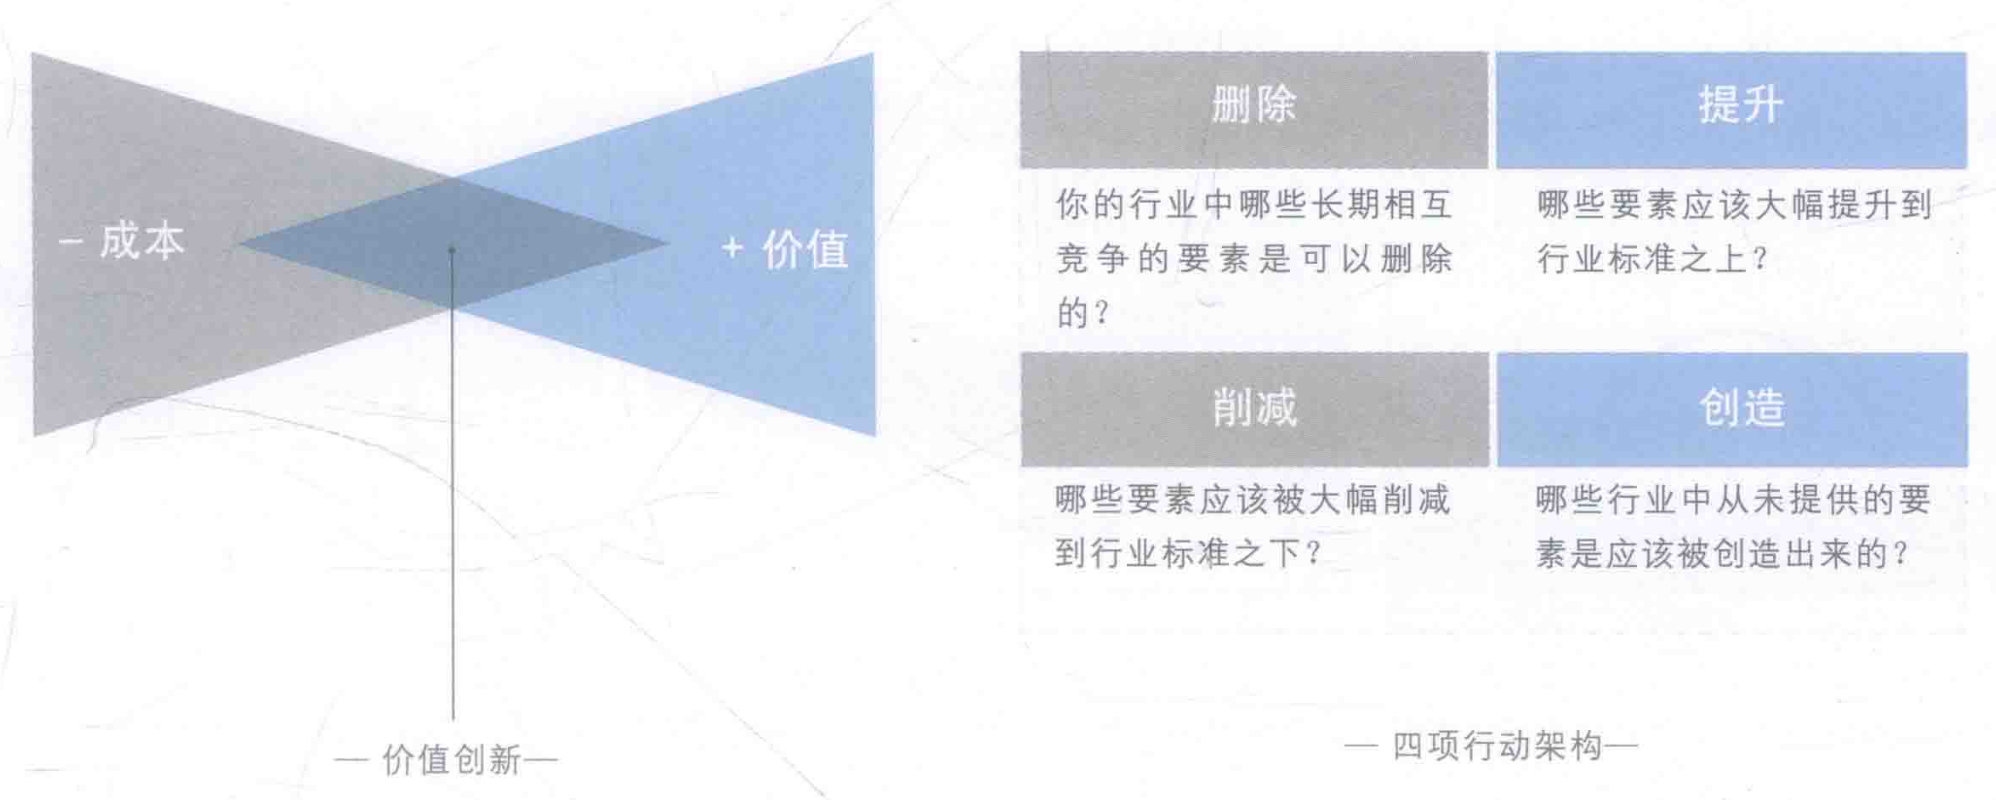
\includegraphics[width=0.6\textwidth]{img/蓝海战略.png}
    \vspace{-0.5em}
\end{figure}

整合蓝海战略框架和商业模式画布
\begin{itemize}
    \item 商业模式右半部关注价值、聚焦客户,左半部分关注成本和基础设施。右侧的改变回对左半部分产生影响
    \item 蓝海战略强调在增加价值的同时减少成本,通过删除和消减低价值产品或服务来降低成本,通过提升和创造对成本影响弱的高价值功能或服务来实现
    \item 二者的整合使得使用“四项行动架构”分析时能够更好地识别这些行动对商业模式其它模块的影响
\end{itemize}

\begin{figure}[H]
	\centering
	\vspace{-0.5em}
	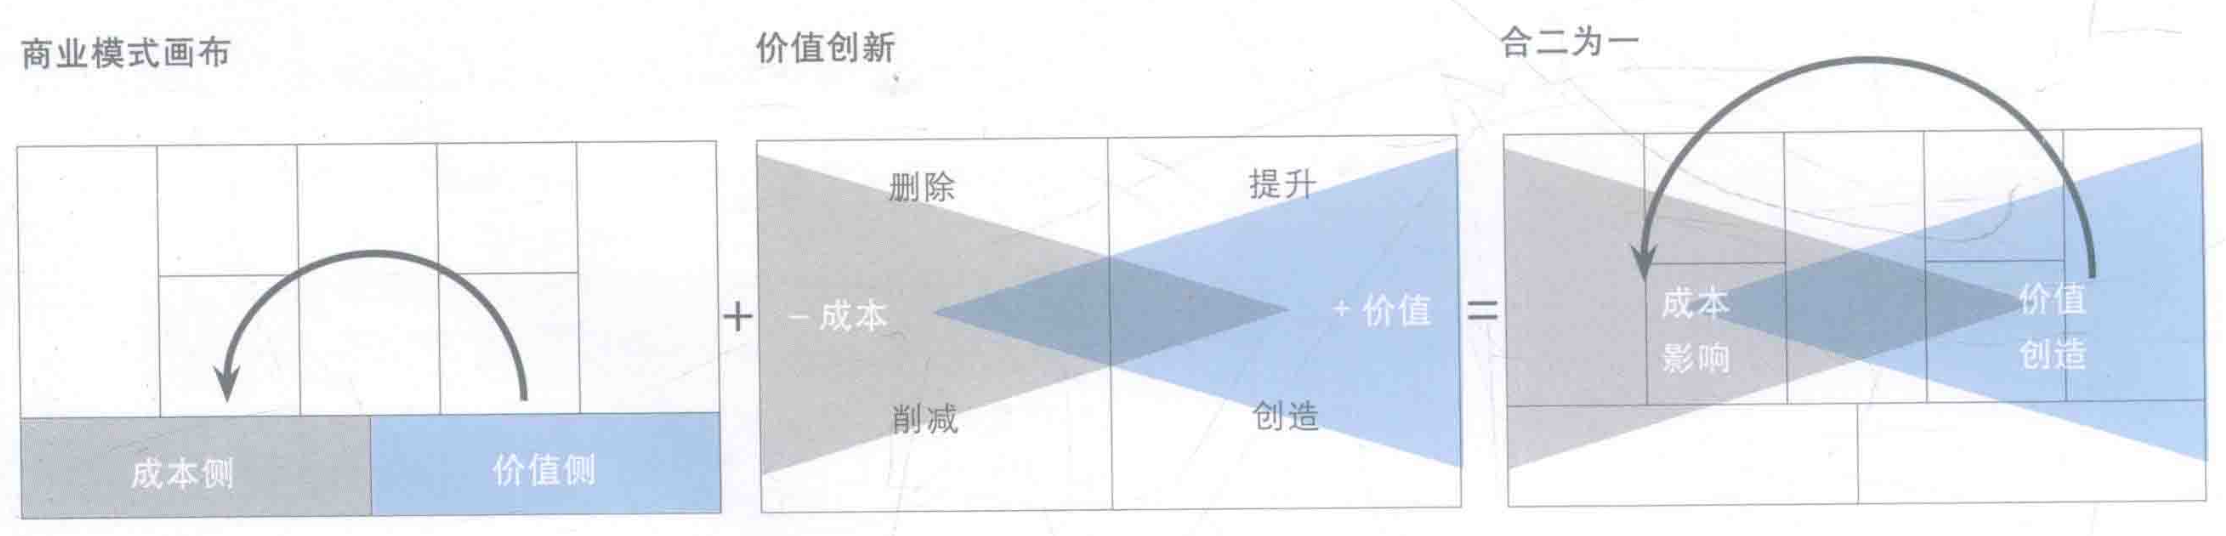
\includegraphics[width=0.9\textwidth]{img/整合蓝海战略框架和商业模式画布.png}
    \vspace{-0.5em}
\end{figure}

例:太阳马戏团
\begin{figure}[H]
	\centering
	\vspace{-0.5em}
	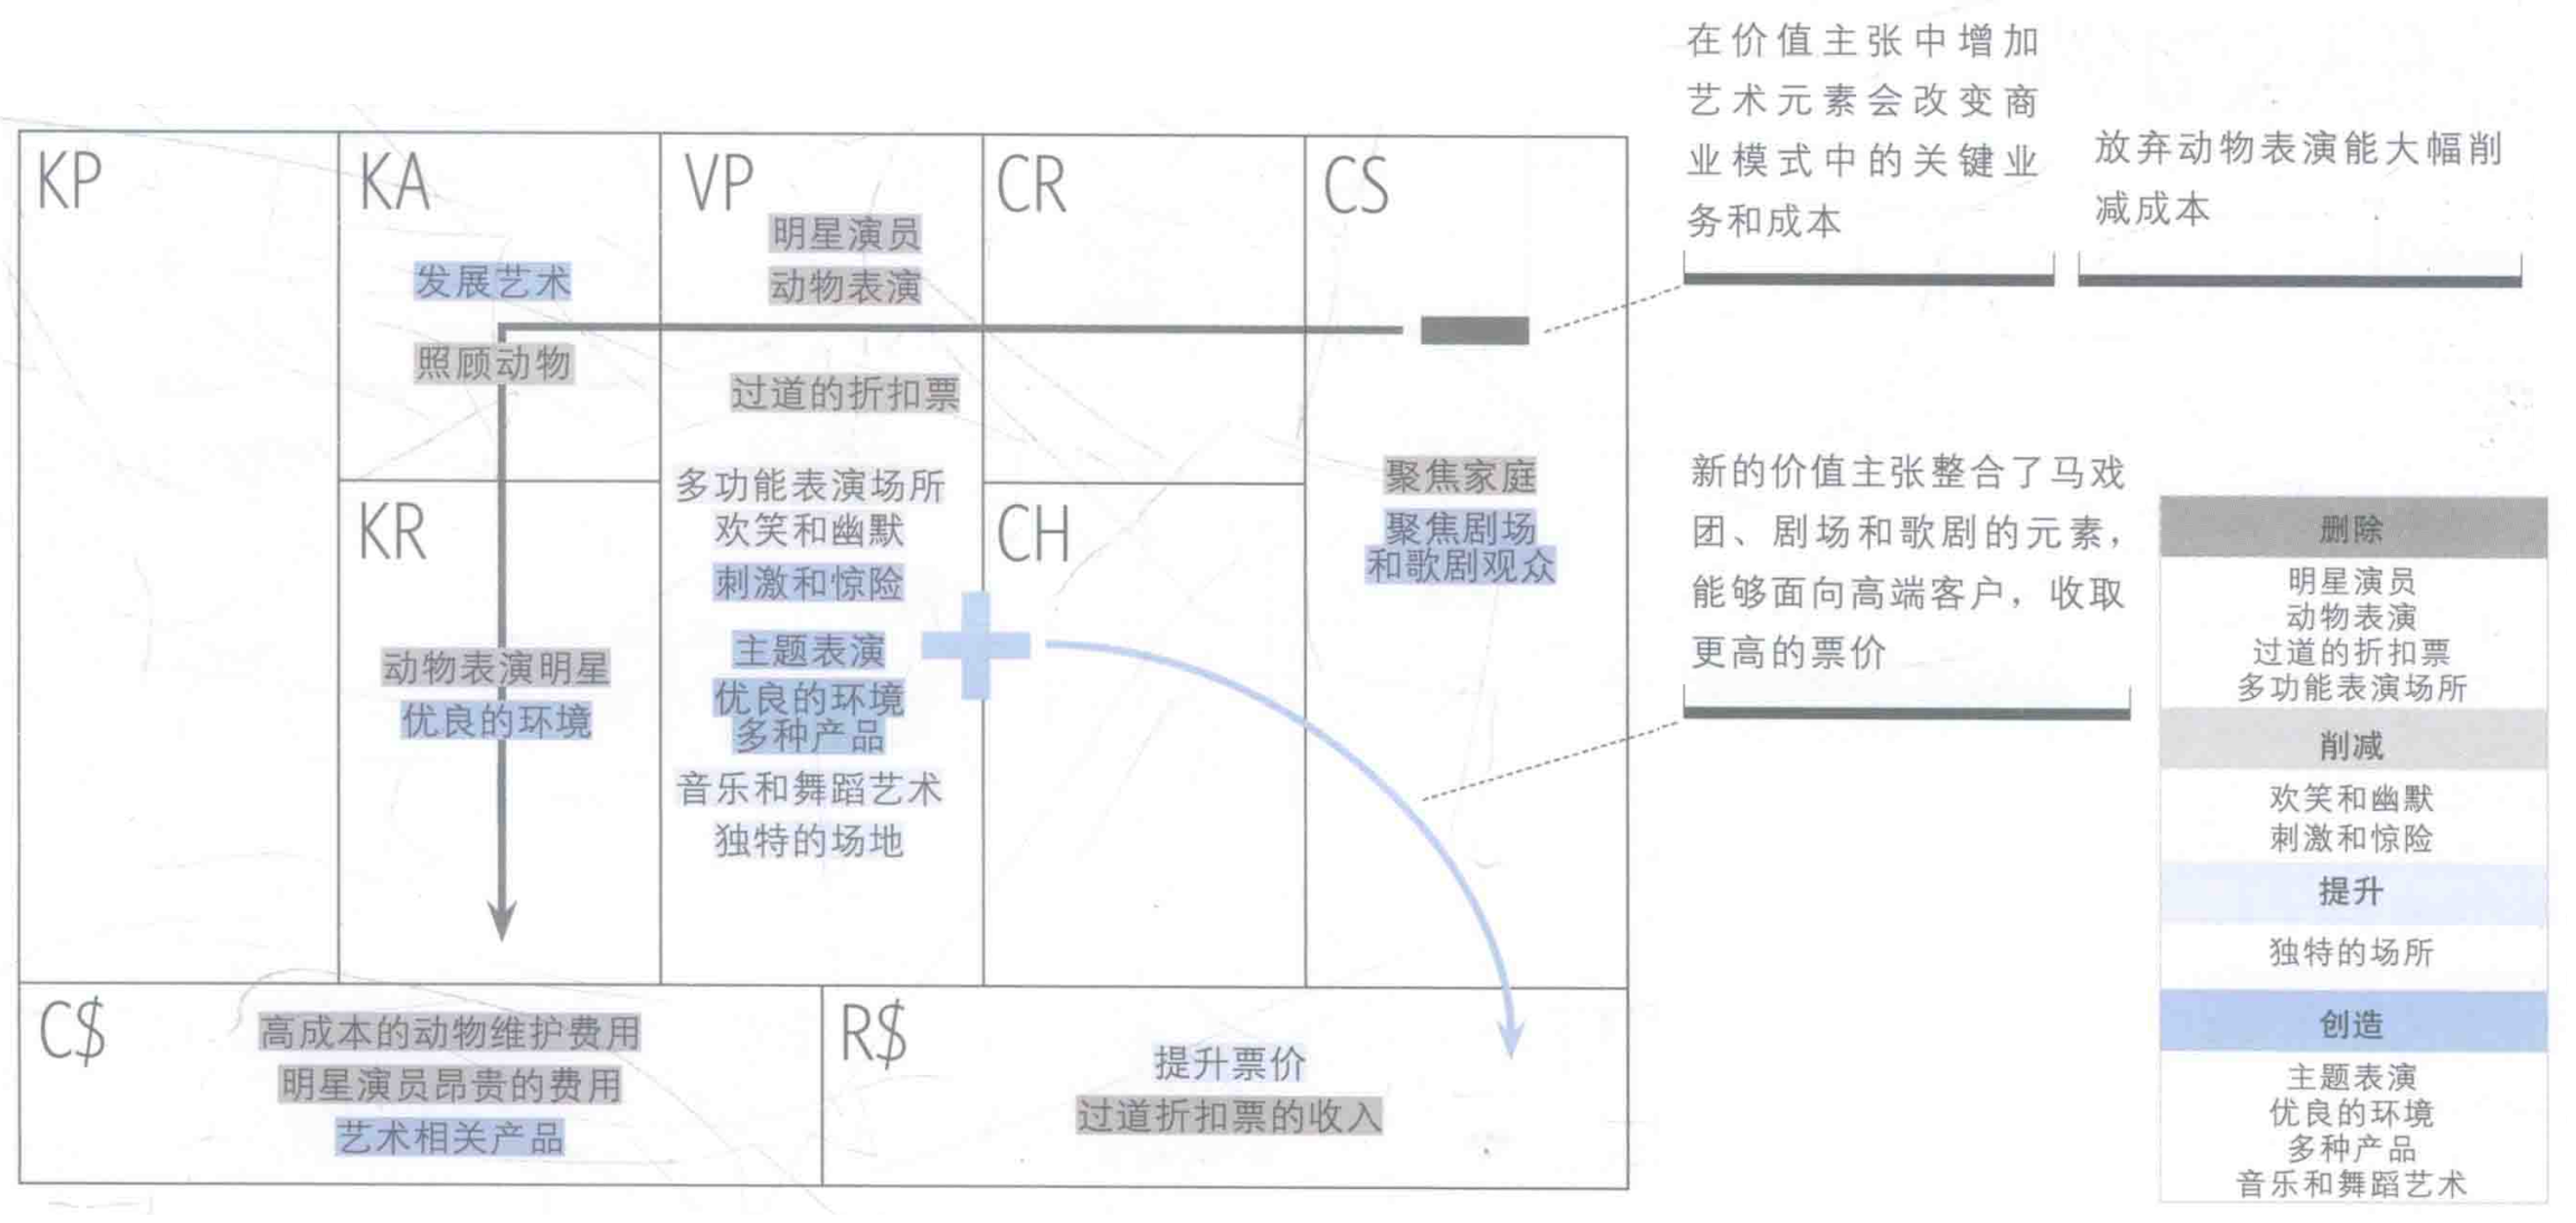
\includegraphics[width=0.85\textwidth]{img/太阳马戏团.png}
    \vspace{-0.5em}
\end{figure}

通过四项行动架构探究画布
\begin{figure}[H]
	\centering
	\vspace{-0.5em}
	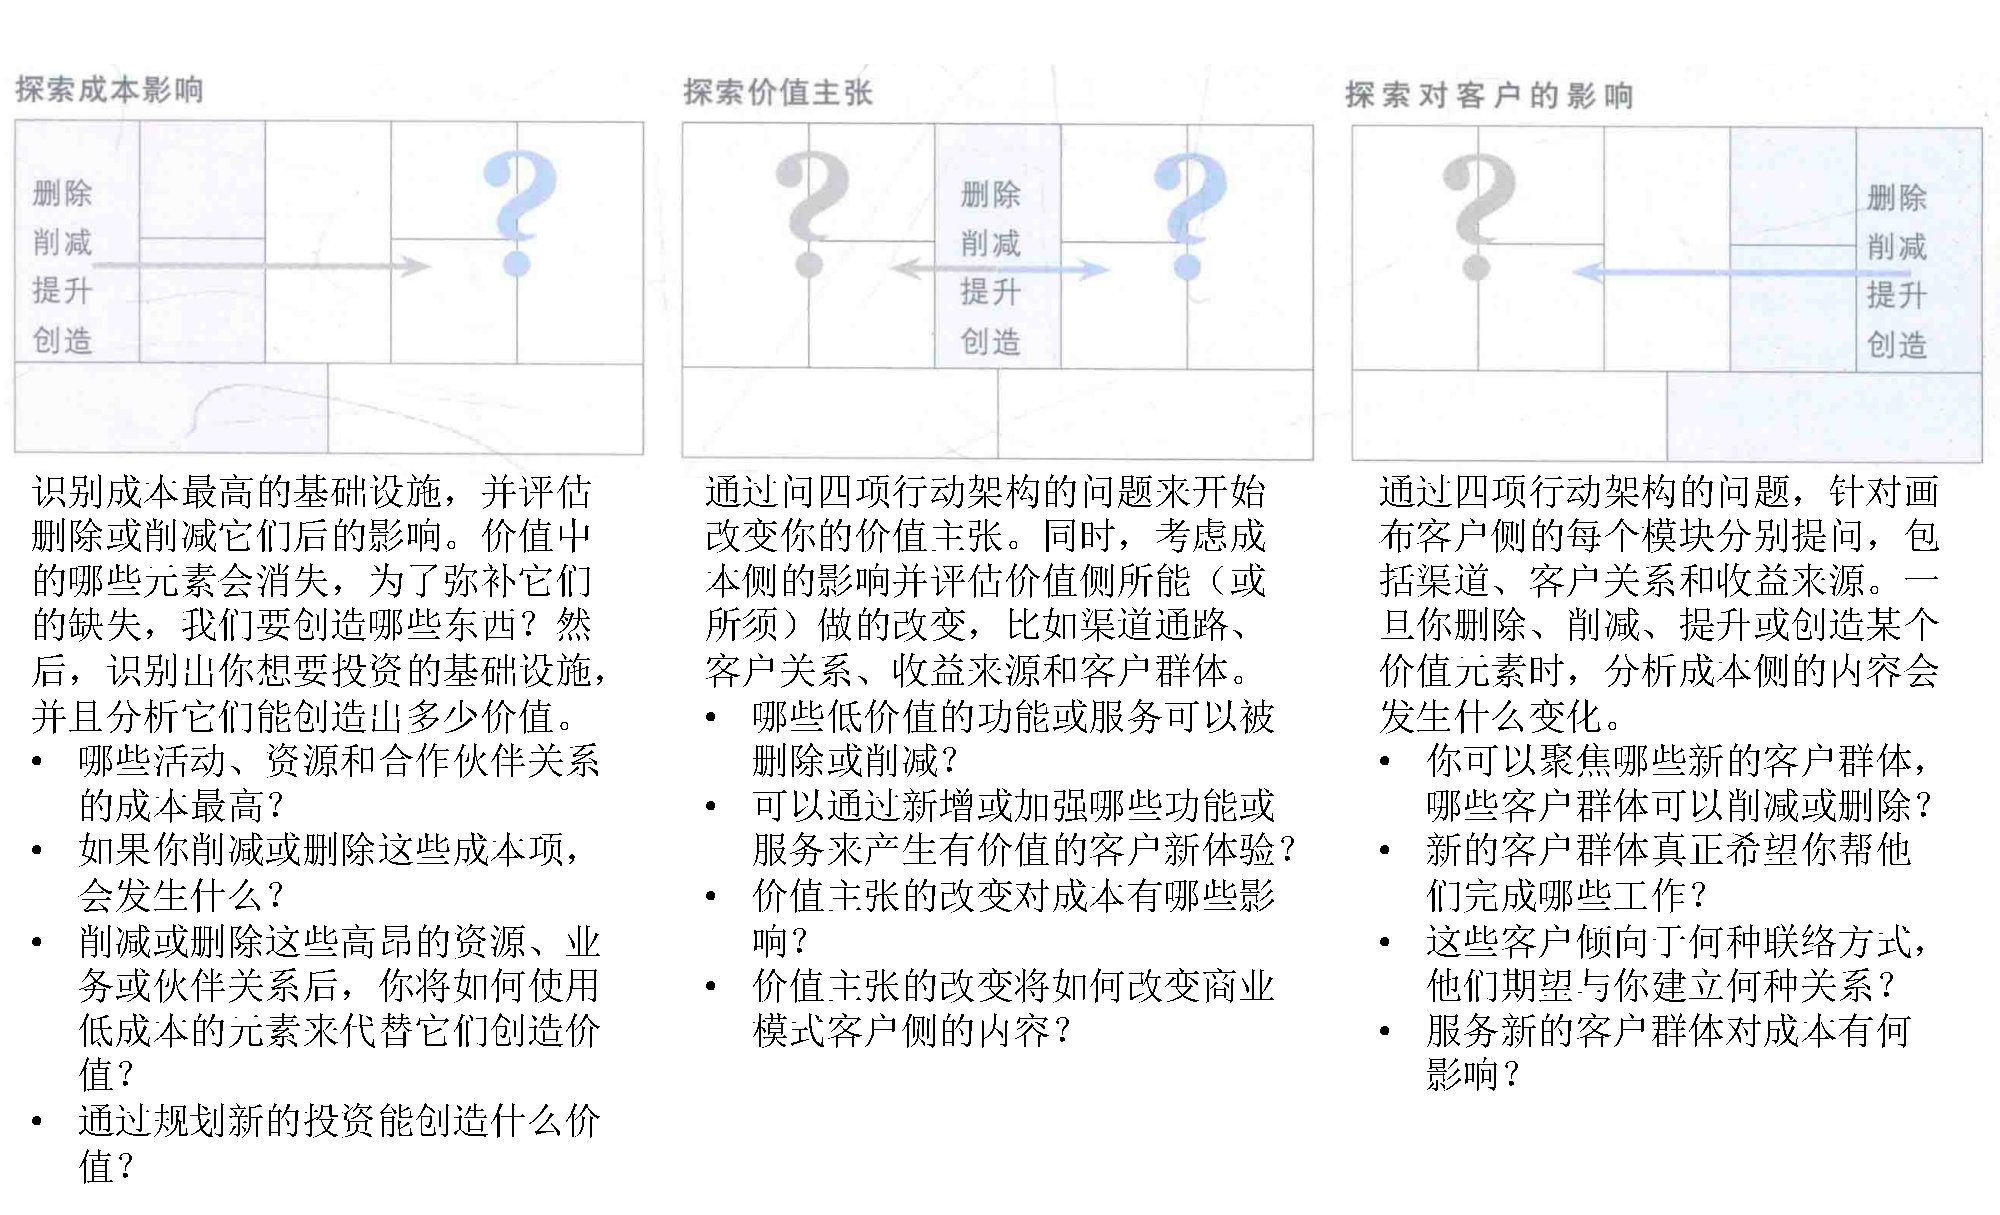
\includegraphics[width=\textwidth]{img/通过四项行动架构探究画布.pdf}
    \vspace{-0.5em}
\end{figure}


\subsection{管理多种商业模式}
成功应对如何在实施和管理新商业模式的同时维持现有的商业模式这个挑战的组织被称为:二元组织。

\begin{itemize}
    \item 组织的艰巨任务:如何在实施和管理新商业模式的同时维持现有的商业模式
    \begin{itemize}
        \item 将新商业模式剥离成一个独立的实体,或者成立独立的业务单元,或维持现状
        \item 拆分商业模式:基础服务、客户关系、新业务
    \end{itemize}
    \item 衡量是否拆分的双变量
    \begin{itemize}
        \item 两种模式冲突的严重程度
        \item 战略上的相似性
        \item 风险是值得我们考感的第三个变量。新的商业模式有多大风险会对现有的模式产生负面的影响,无论是品牌形象、收入、法律责任,还是其他方面
    \end{itemize}
\end{itemize}

\begin{figure}[H]
	\centering
	\vspace{-0.5em}
	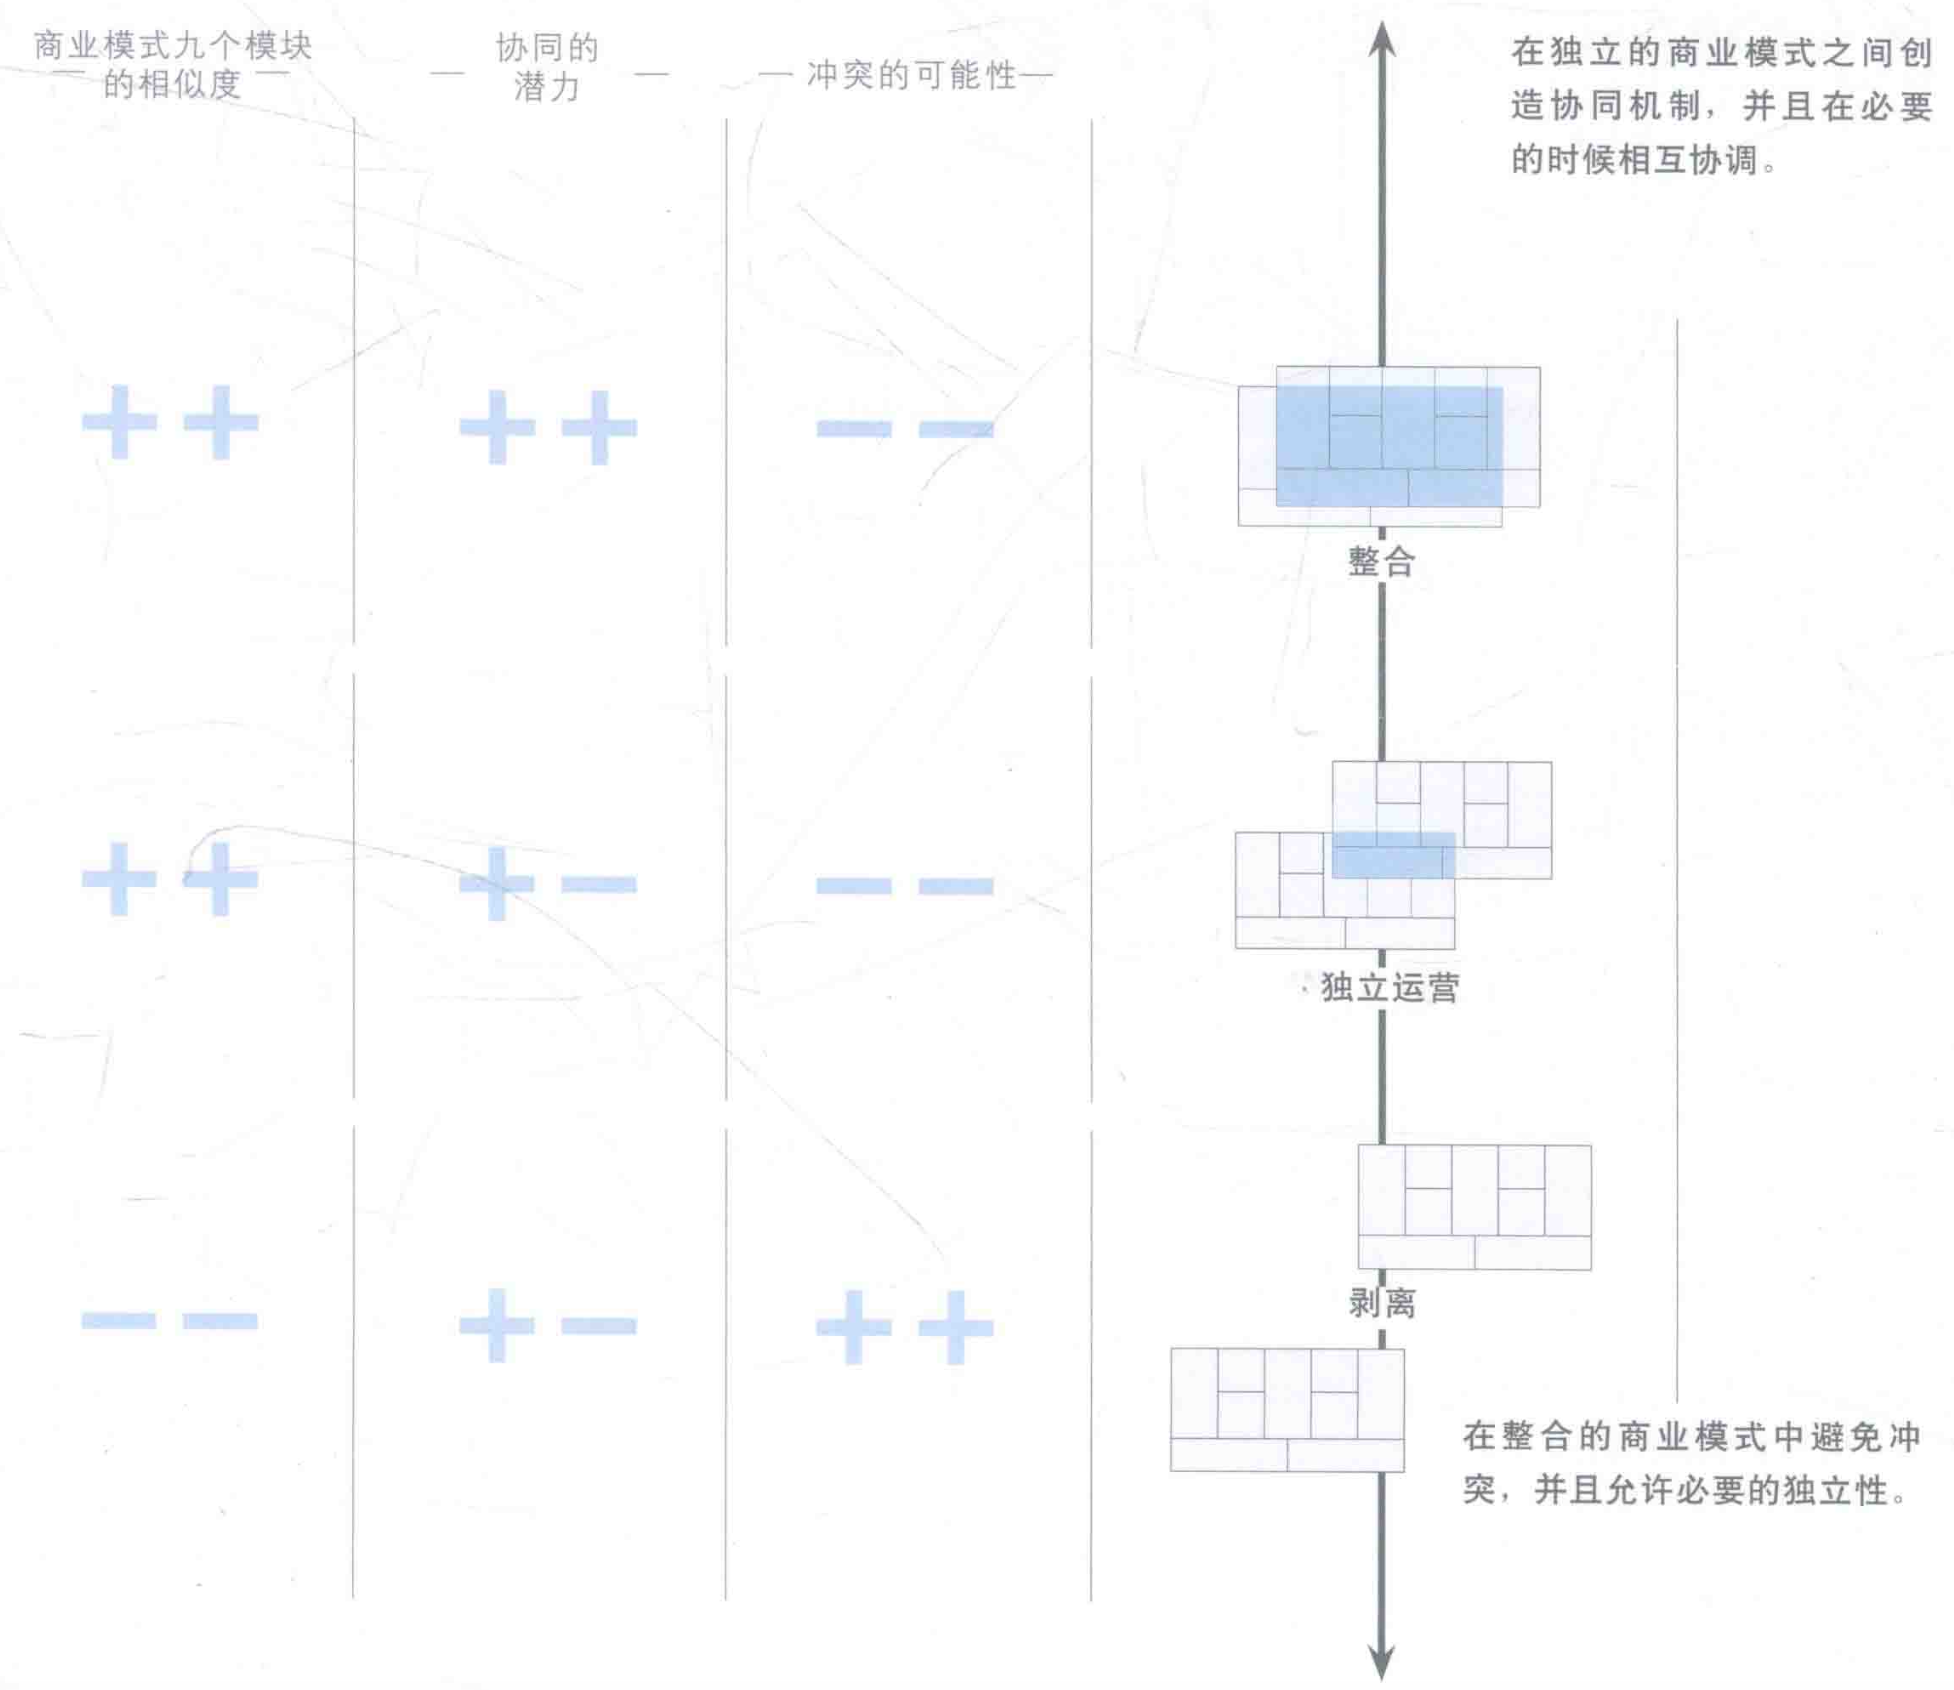
\includegraphics[width=0.6\textwidth]{img/管理多种商业模式.png}
    \vspace{-0.5em}
\end{figure}

例:SMH(后改名为SWATCH,斯沃琪)的SWATCH品牌的独立运营模式
\begin{figure}[H]
	\centering
	\vspace{-0.5em}
	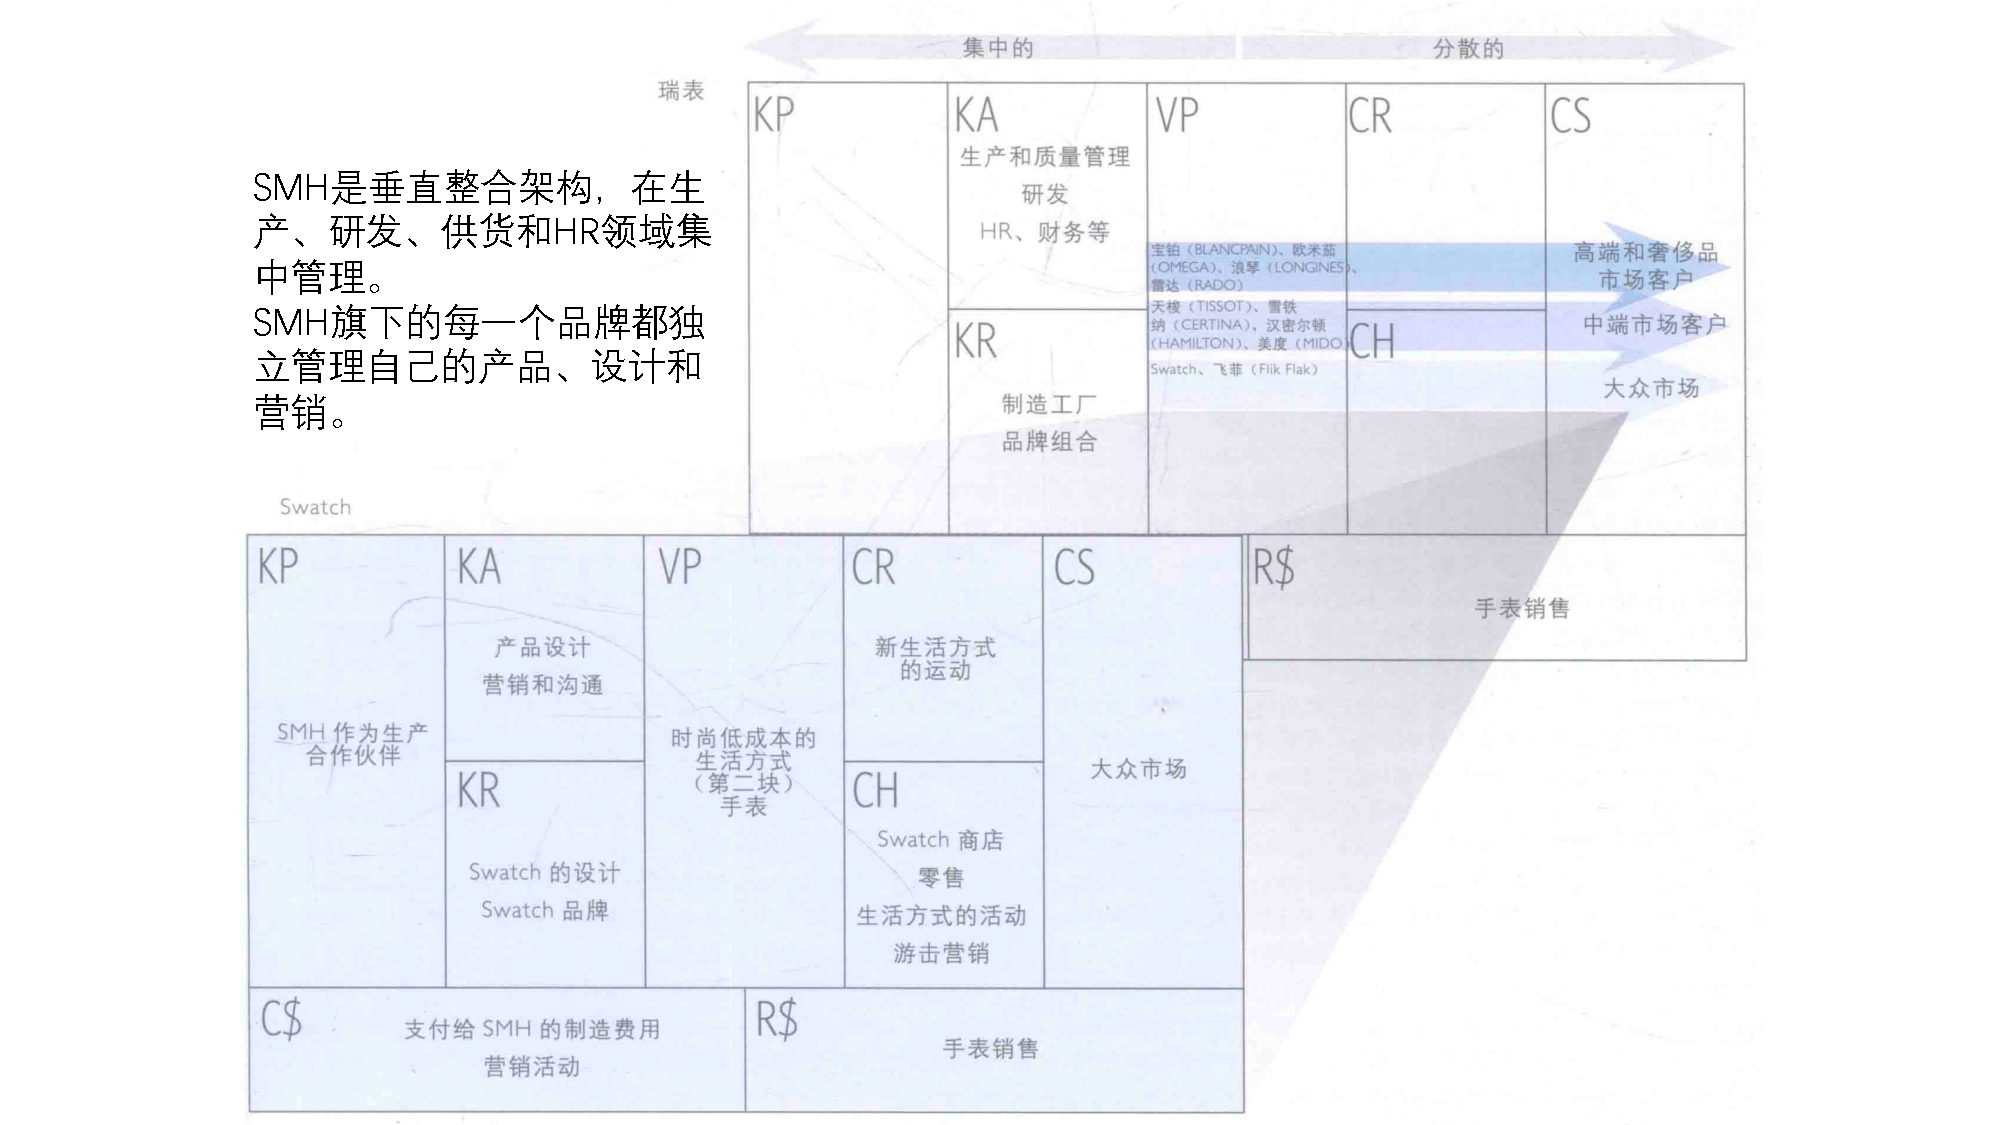
\includegraphics[width=0.7\textwidth]{img/SMH的SWATCH品牌的独立运营模式.pdf}
    \vspace{-0.5em}
\end{figure}

例:雀巢公司的咖啡商业模式组合
\begin{figure}[H]
	\centering
	\vspace{-0.5em}
	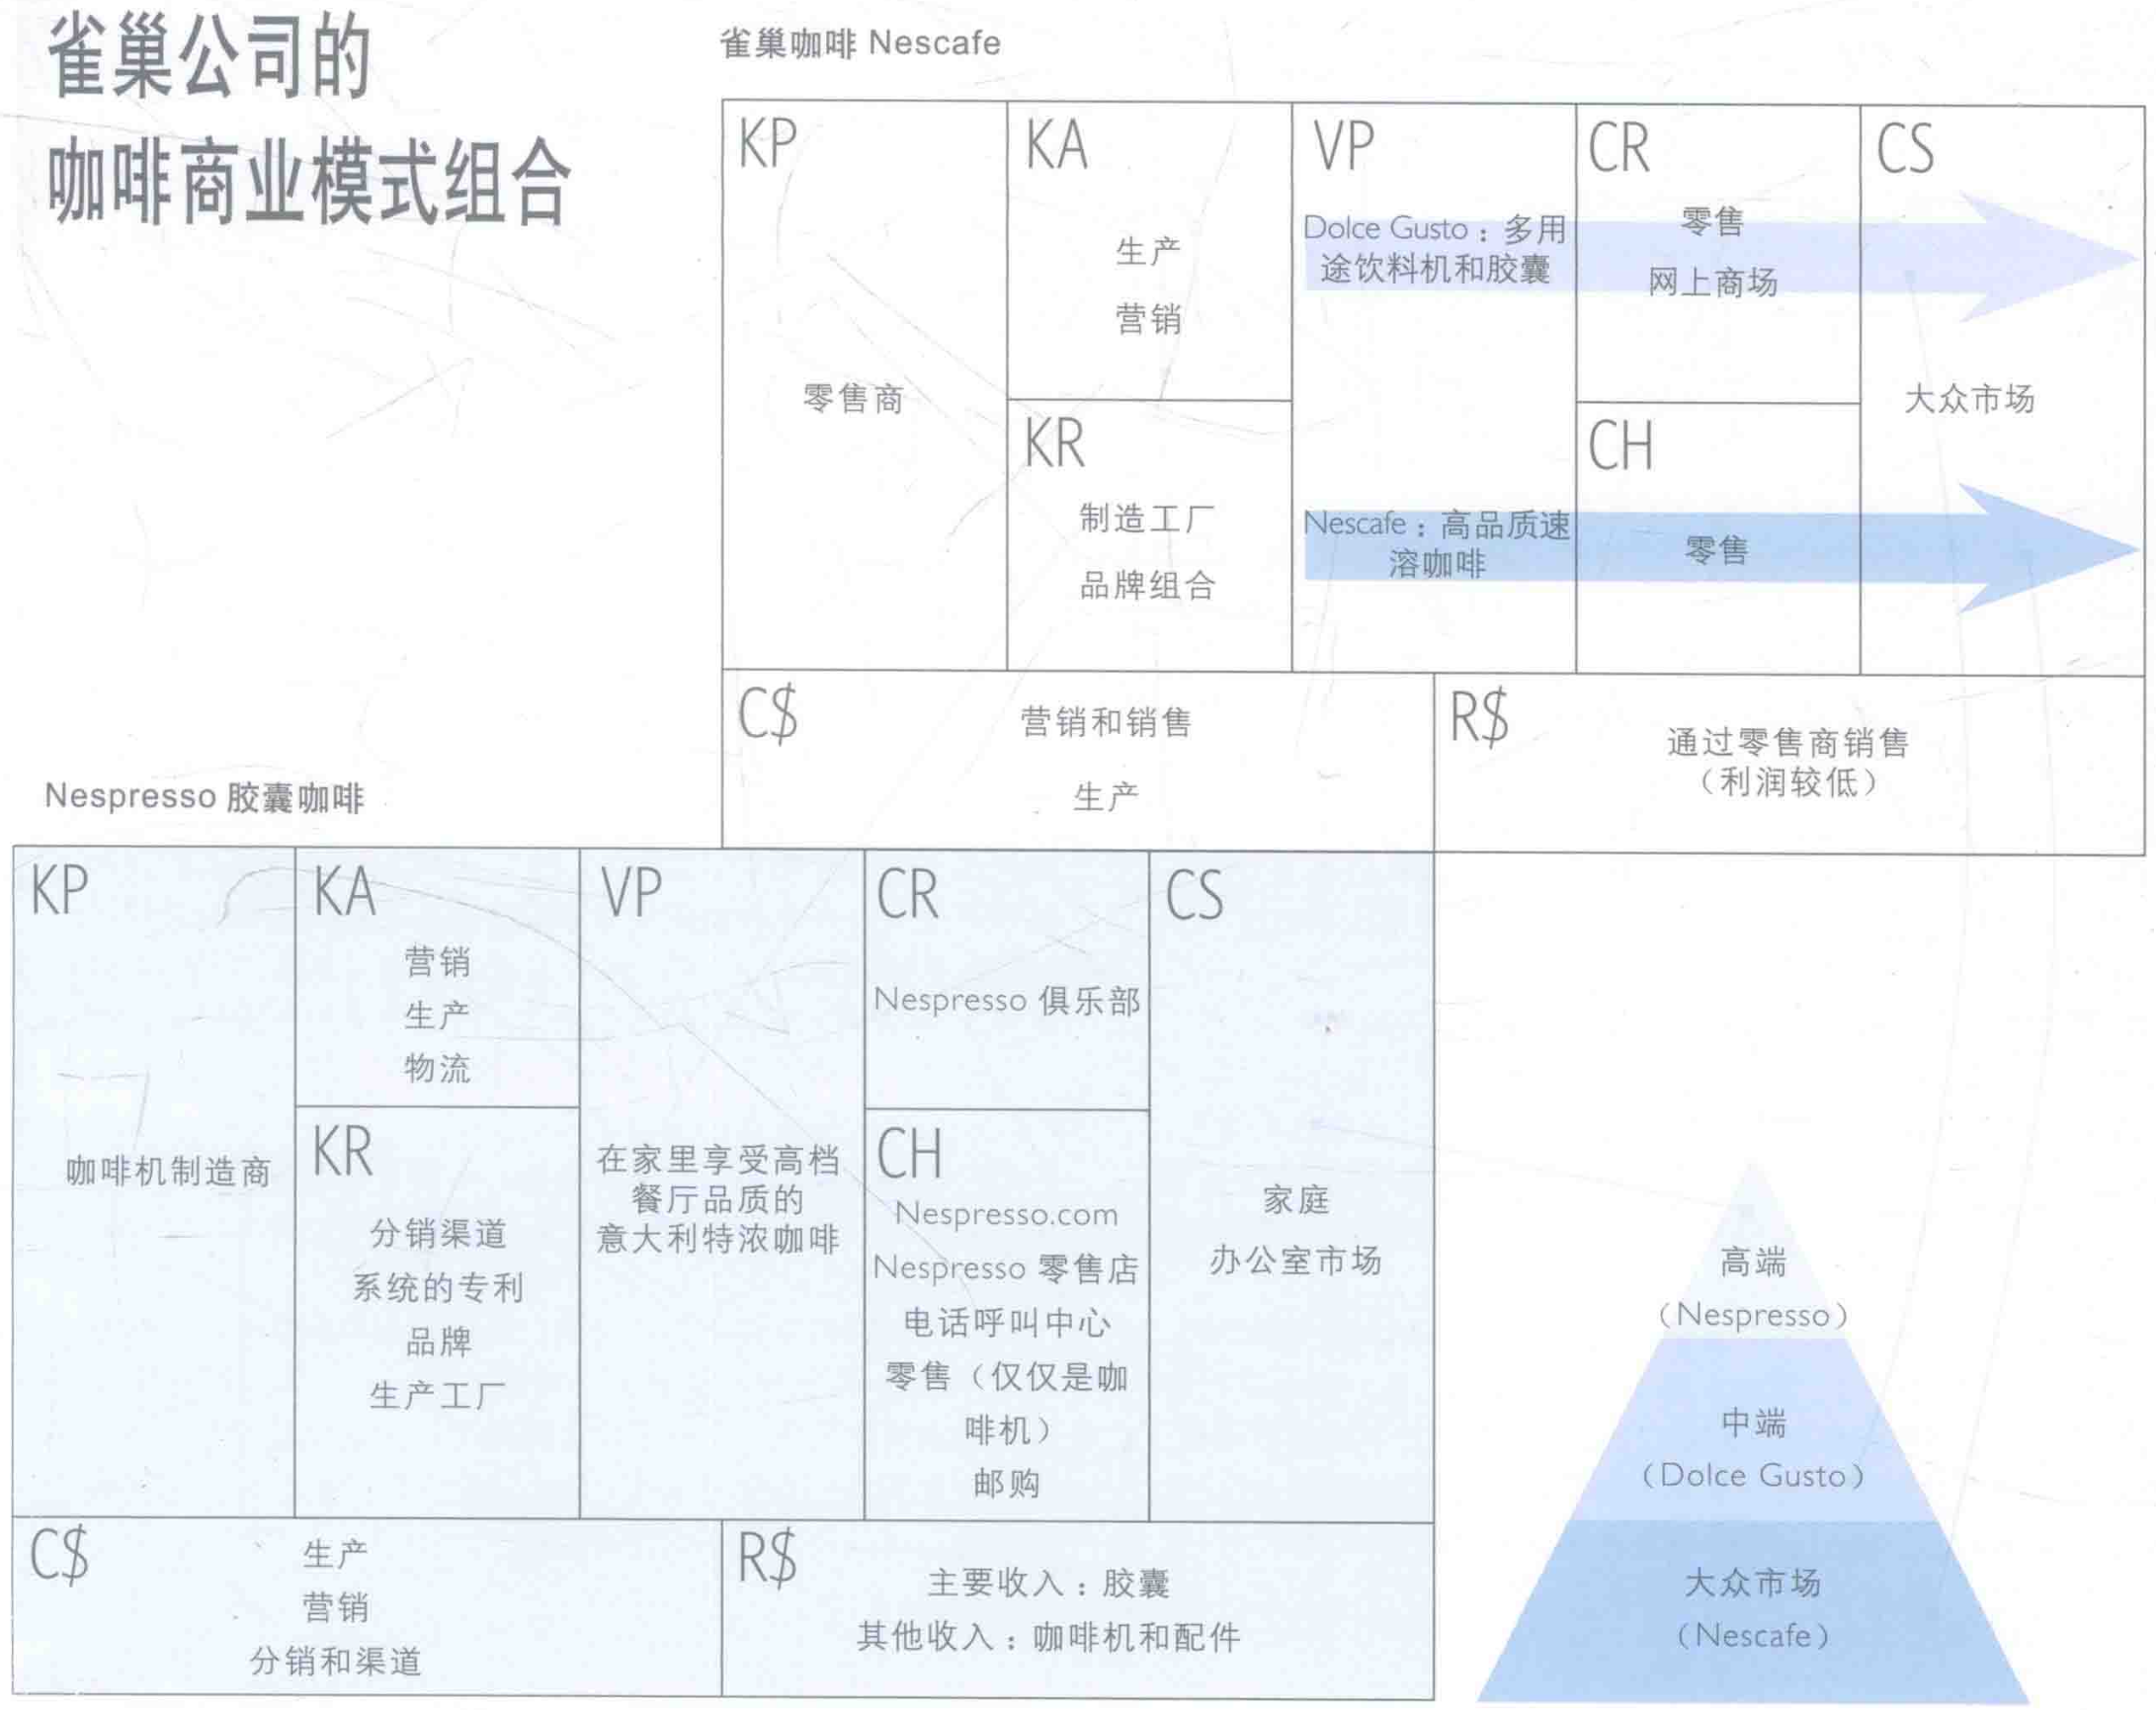
\includegraphics[width=0.7\textwidth]{img/雀巢公司的咖啡商业模式组合.png}
    \vspace{-0.5em}
\end{figure}

例:戴姆勒公司Car2go的商业模式
\begin{figure}[H]
	\centering
	\vspace{-0.5em}
	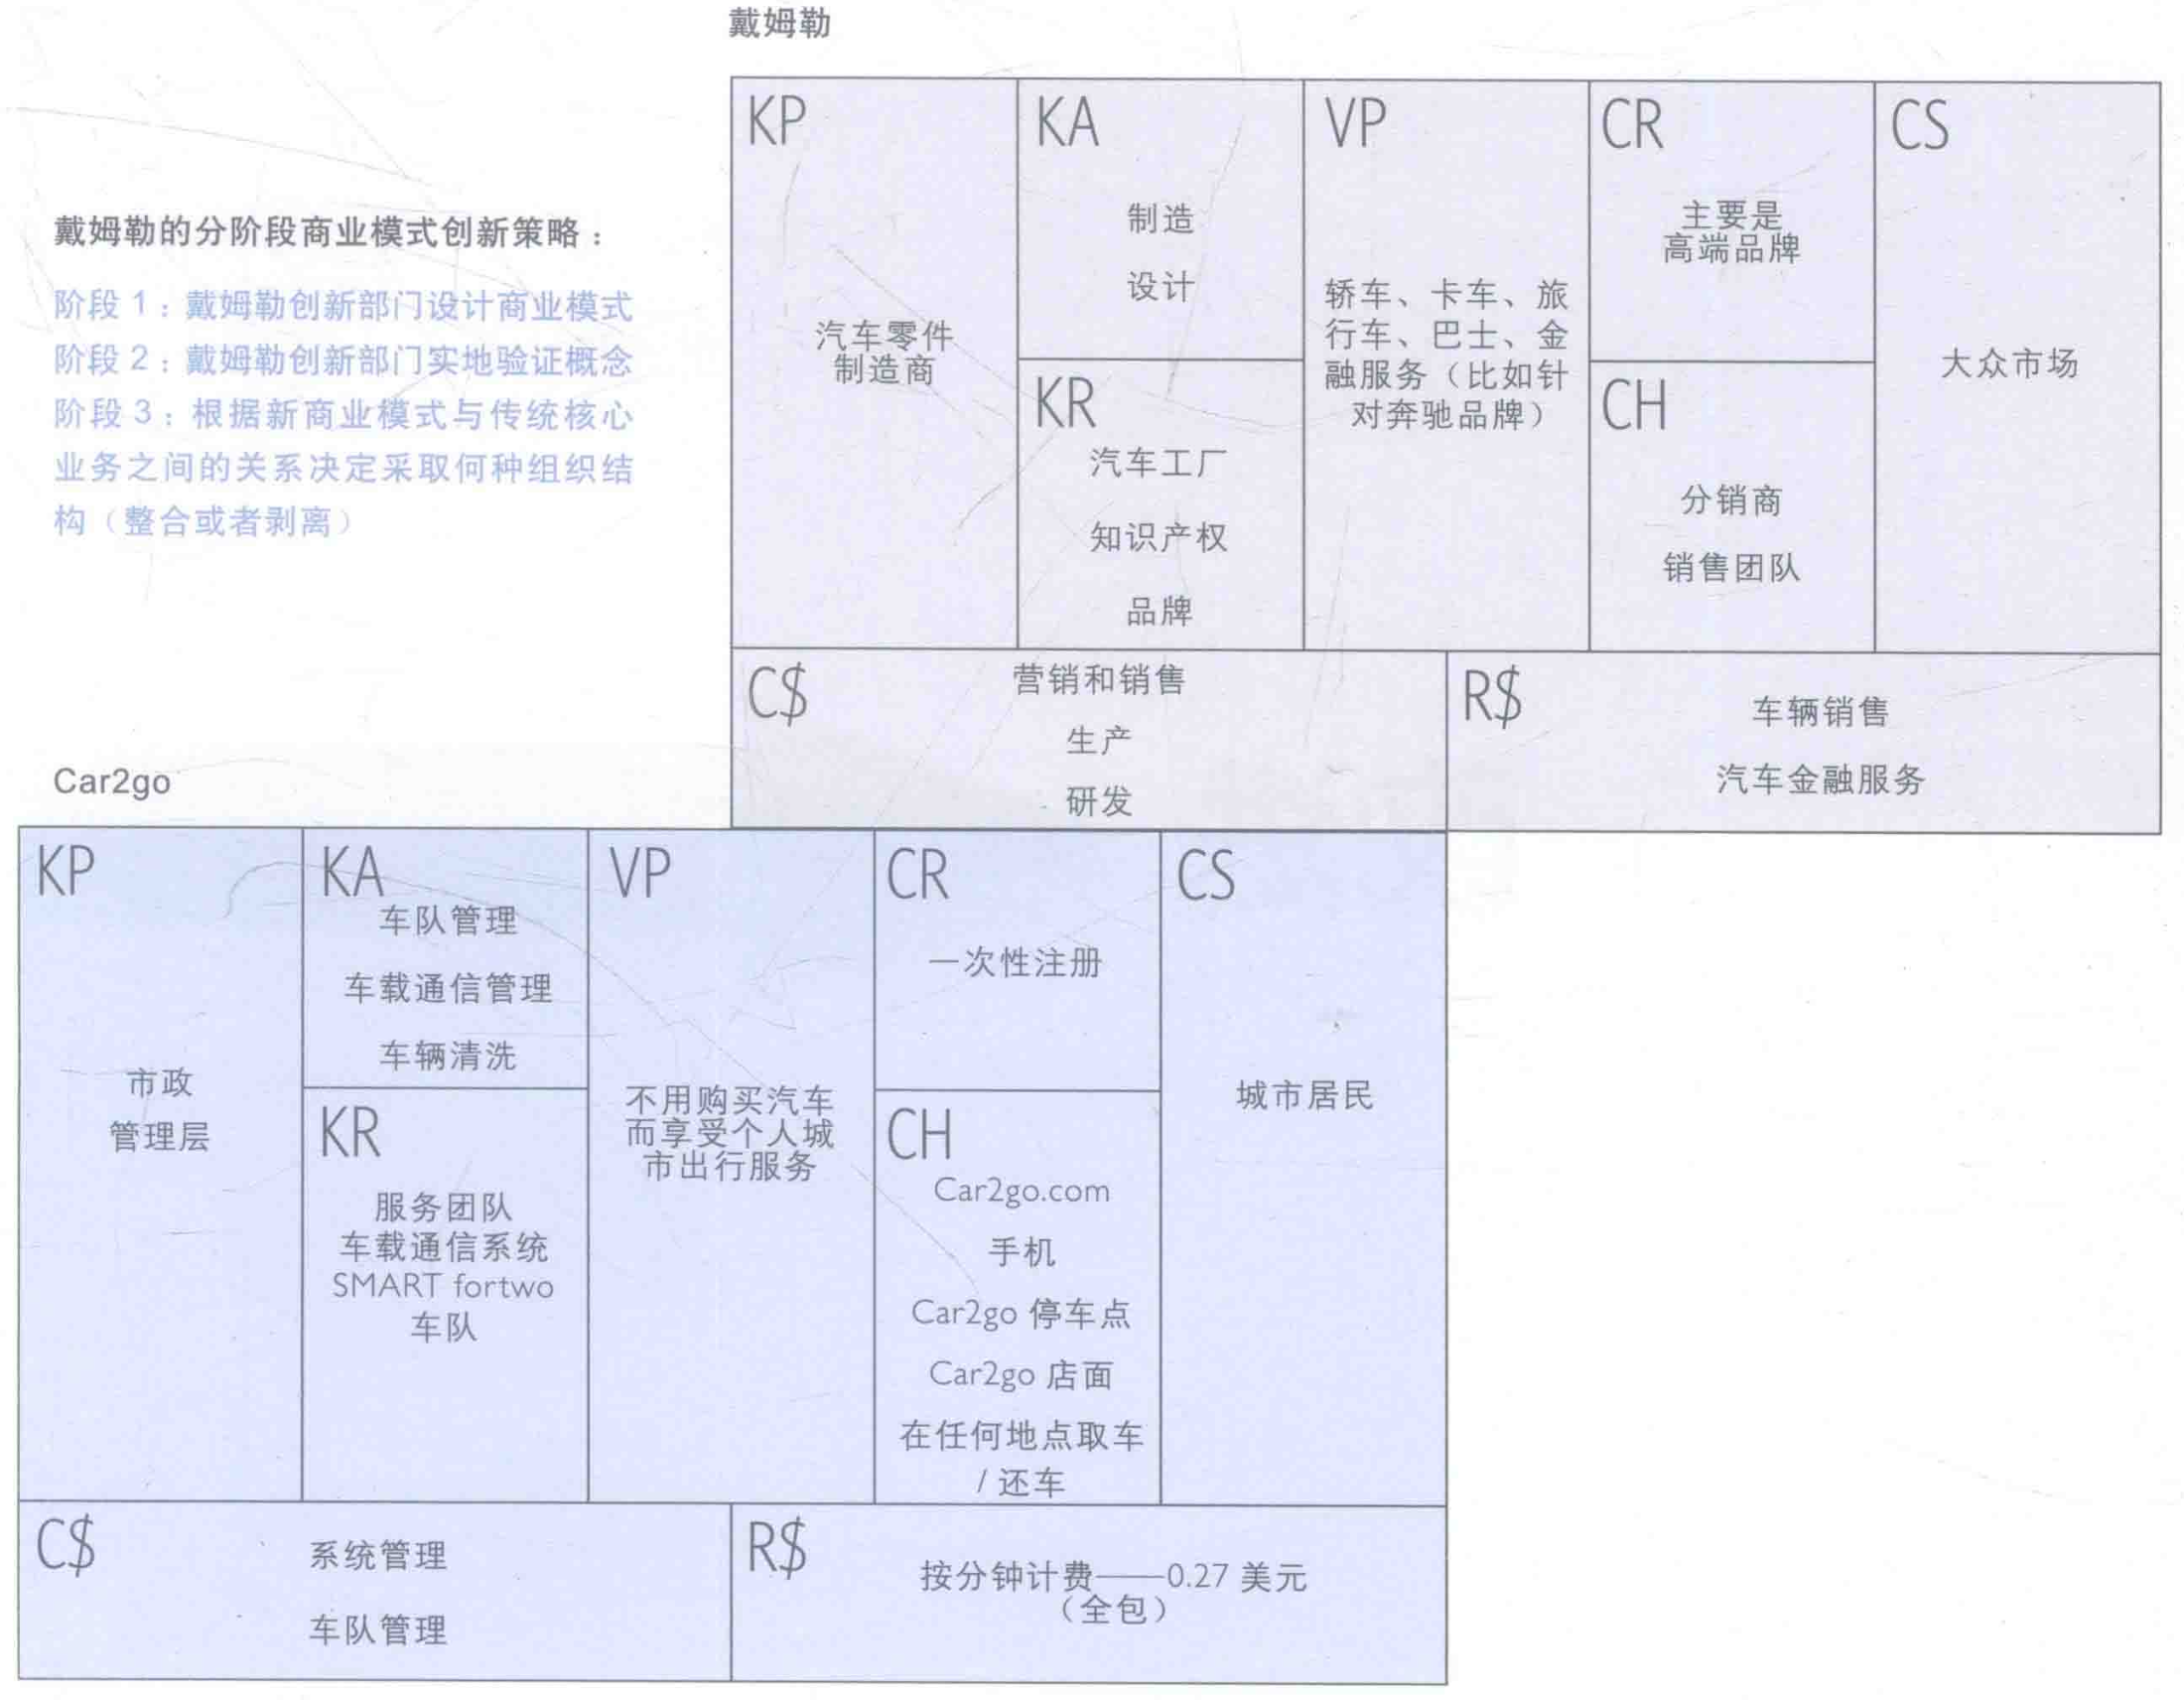
\includegraphics[width=0.7\textwidth]{img/戴姆勒公司Car2go的商业模式.png}
    \vspace{-0.5em}
\end{figure}